\section{Self-Supervised Learning}
Self-Supervised Learning (SSL) is, unlike supervised learning, learning information about some data without any labels. The way SSL is not unsupervised is by defining a learning objective based on the underlying structure of the data itself, this is called a pretext task.
In general this in done by predicting any unobserved or hidden part of the input data using only the observed or unhidden part of the input data. 
For natural langues processing (NLP) one way to do so is by hide words and try to predict the hidden words. a common way to do so is using masks. When using masks the objective is to predict the masked word from the surrounding words. This encourage the model to learn the relationships between different words, which then can be utilized in a range of downstream tasks. This could for example be translating text, summarizing, or generating text. 
In computer vision (CV) the same approach, predicting masked patches of an image or representation, have been used in models such as MAE and BYOL [KILDER]. Other approaches are also common in CV, for example using the objective of mapping two versions of the same image to the same representations.
Even though the idea of SSL is very similar across different domains, such as NLC, CV, or audio, their algorithms and objectives are very different. This is mainly because they were developed with a single domain in mind. A framework which is created with multiple domains in mind is data2vec.

\todo[inline]{Maybe add some from data2vec article into \\This is mainly from Meta Cookbook}

\section{Data2vec}
Data2vec is a framework which is created to get closer to one leaning method for all SSL problems. The version of data2vec which is used in this project has implemented a method which works on either speech, NLP, or CV. The method used combines masked prediction with the learning of latent target representations generalized by using multiple network layers as targets. This is done by having a student mode and a teacher mode. First the input data is masked and encoded to create a representation of the masked input. The unmasked input data is then encoded and parameterized as an exponential moving average to create the training targets. Now the learning objective is for the student to predict the target representations, given a partial view of the input. This is illustrated on \Cref{fig:data2vec_ilu}.

\begin{figure}
    \centering
    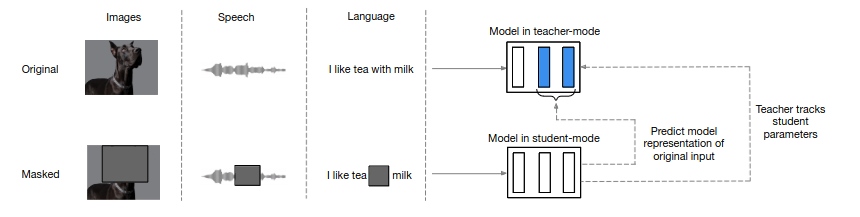
\includegraphics[width=\textwidth]{incl/img/data2vec/data2vec_ilu.png}
    \caption{An illustration of how data2vec works on different data types, using the same process. The model creates a representation of the original input data and then a masked version of the input.}
    \label{fig:data2vec_ilu}
\end{figure}

% To create the representations on the different data types models there are used encoders specified to the datatype.

The way the model is trained is to predict the representation of the unmasked sample, only knowing the encoding of the masked sample.

% Herfra, I dont know....
In the teacher mode the encoding is parameterized by an exponential moving average of the model parameters where the weights of the model in target-mode \(\Delta\) are
\begin{align}
    \Delta \leftarrow \tau \Delta + (1-\tau)\theta,
\end{align}
where \(\theta\) is the model parameters, and \(\tau\) is linearly increasing from \(\tau_0\) to \(\tau_e\) over the first \(\tau_n\) updates and are constant hereafter. This makes the teacher update more frequently in the beginning of the training when the model is more random and less frequently when good parameters have been learned.

The training targets are constructed from the last \(K\) blocks of parameters from the teacher network at the same time step as the student network. The training target at time step \(t\), for a network with \(L\) blocks in total, is then
\begin{align}
    y_t = \sum_{l=L-K+1}^L \hat{a}_t^l,
\end{align}
where \(\hat{a}_t^l\) is the normalized output of block \(l\) at time step \(t\). The normalizing helps the network not to collapse and layers with high norm to not dominate the target feature. For speech the normalizing used is instance normalizing \cite{ulyanov2016instance} without any learned parameters over the current input sample, this is because the neighboring representations are highly correlated due to small stride over the input data. Whereas for NLP and CV a parameter-less layer normalization \cite{ba2016layer} is used. 